\documentclass{article}

\usepackage{adjustbox}
\usepackage{amsfonts}       % blackboard math symbols
\usepackage{amsmath}
\usepackage{batter_pitcher_2vec}
\usepackage[doi=false,
            eprint=false,
            isbn=false,
            maxbibnames=99,
            sorting=none]{biblatex}        % bibliography
\usepackage{booktabs}       % professional-quality tables
\usepackage[T1]{fontenc}    % use 8-bit T1 fonts
\usepackage{hyperref}       % hyperlinks
\usepackage[utf8]{inputenc} % allow utf-8 input
\usepackage{mathtools}
\usepackage{microtype}      % microtypography
\usepackage{nicefrac}       % compact symbols for 1/2, etc.
\usepackage{subcaption}
\usepackage{tikz}
\usepackage{url}            % simple URL typesetting

\addbibresource{batter_pitcher_2vec.bib}

\title{\texttt{(batter|pitcher)2vec}: statistic-free talent modeling with neural player embeddings}
\date{}

\author{
    Michael A. Alcorn\thanks
    {Personal website: \url{https://sites.google.com/view/michaelaalcorn}\newline
    \hspace*{1.8em}Code: \url{https://github.com/airalcorn2/batter-pitcher-2vec}} \\
    Red Hat, Inc.\\
    Chicago, IL 60615 \\
    \texttt{michaelaalcorn@gmail.com} \\
}

\begin{document}

\maketitle

\begin{abstract}

This paper introduces \texttt{(batter|pitcher)2vec}, a neural network algorithm inspired by \texttt{word2vec} that learns distributed representations of Major League Baseball players. The representations are discovered through a supervised learning task that attempts to predict the outcome of an at-bat (e.g., strike out, home run) given a specific batter and pitcher. The learned representations qualitatively appear to better reflect baseball intuition than traditional baseball statistics, for example, by grouping together pitchers who rely primarily on pitches with dramatic movement. Further, like \texttt{word2vec}, the representations possess intriguing algebraic properties; for example, capturing the fact that Bryce Harper might be considered Mike Trout's left-handed dopplegänger. Lastly, \texttt{(batter|pitcher)2vec} is significantly more accurate at modeling future at-bat outcomes for previously unseen matchups than simpler approaches.

\end{abstract}

\section{Introduction}

Baseball is notorious for its culture of statistical bookkeeping. The depth and breadth of baseball statistics allows fans and professionals alike to compare players and forecast outcomes with varying degrees of accuracy. Although many traditional baseball statistics can be quite informative and useful, they can also be somewhat arbitrary and thus may not accurately reflect the true talent of any given player.

The field of Sabermetrics was developed in an effort to address some of the inherent limitations of standard baseball statistics. For example, Wins Above Replacement (WAR) "offers an estimate to answer the question, 'If this player got injured and their team had to replace them with a freely available minor leaguer or a AAAA player from their bench, how much value would the team be losing?'" \parencite{WAR}. However, the WAR formula (\ref{eqn:war}) is, itself, somewhat ad hoc, reflecting the intuition of the statistic's designer(s):

\begin{equation}
\label{eqn:war}
WAR = \frac{BR + BRR + FR + PA + LA + RR}{RPW}
\end{equation}

where $BR$ is batting runs, $BRR$ is base running runs, $FR$ is fielding runs, $PA$ is a positional adjustment, $LA$ is a league adjustment, $RR$ is replacement runs, and $RPW$ is runs per win.

Whereas the WAR statistic uses a combination of conventional baseball statistics to quantify an individual player's impact on his team's overall record, the Player Empirical Comparison and Optimization Test Algorithm (PECOTA) attempts to forecast player performance by identifying a neighborhood of players with historically similar statistics (both traditional and of the Sabermetrics variety) and then performing an age correction \parencite{PECOTA}. However, the neighborhoods produced by PECOTA are proprietary, which precludes deeper investigation by the community.

When scouts assess the talent of a player, they do not simply count up the number of times the player made it to first base or struck out. They consider the player's tendencies in a number of different contexts. For example, a scout might notice that a certain left-handed batter tends to ground out to third base when facing left-handed curveball pitchers. Or that a certain right-handed fastball pitcher tends to struggle against short right-handed batters. An algorithm capable of learning these subtleties would be a valuable tool for assessing player talent.

The task of extracting informative measures of talent for Major League Baseball (MLB) players is surprisingly similar to the task of constructing useful word embeddings in the field of natural language processing. Words, like MLB players, can be considered distinct elements in a set, and one common way to represent such categorical data in machine learning algorithms is as one-hot encodings. A one-hot encoding is an $N$-dimensional vector (where $N$ is the number of elements in the set) consisting entirely of zeros except for a single one at the location corresponding to the element's index. For example, the one-hot encodings for a vocabulary consisting of the words \{"dog", "cat", "constitutional"\} might be $\begin{bsmallmatrix} 1 & 0 & 0 \end{bsmallmatrix}$, $\begin{bsmallmatrix} 0 & 1 & 0 \end{bsmallmatrix}$, and $\begin{bsmallmatrix} 0 & 0 & 1 \end{bsmallmatrix}$, respectively.

One drawback of one-hot encodings is that each vector in the set is orthogonal to and equidistant from every other vector in the set; i.e., every element in the set is equally similar (or dissimilar) to every other element in the set. Words, however, \emph{do} exhibit varying degrees of semantic similarity. For example, the words "dog" and "cat" are clearly semantically more similar than the words "dog" and "constitutional". Word embeddings mathematically encode such similarity patterns as geometric properties (e.g., cosine similarity or Euclidean distance), and using these representations generally leads to more computationally efficient learning algorithms \parencite{Bengio2003}.

Perhaps the most famous word embedding algorithm is \texttt{word2vec} \parencite{Mikolov2013}, a neural network that learns distributed representations of words in a supervised setting. The \texttt{word2vec} algorithm can take two different forms: (1) the continuous bag-of-words model (CBOW) and (2) the skip-gram model (see Figure~\ref{fig:word2vec}). The CBOW model attempts to predict a word ($w_t$) given some surrounding words (e.g., $w_{t-1}$ and $w_{t+1}$, although the context can be larger). In contrast, the skip-gram model attempts to predict the surrounding words of a given central word.

\begin{figure}[h]
\captionsetup[subfigure]{labelformat=empty}
\centering

    \begin{subfigure}[t]{0.45\textwidth}
    \centering
    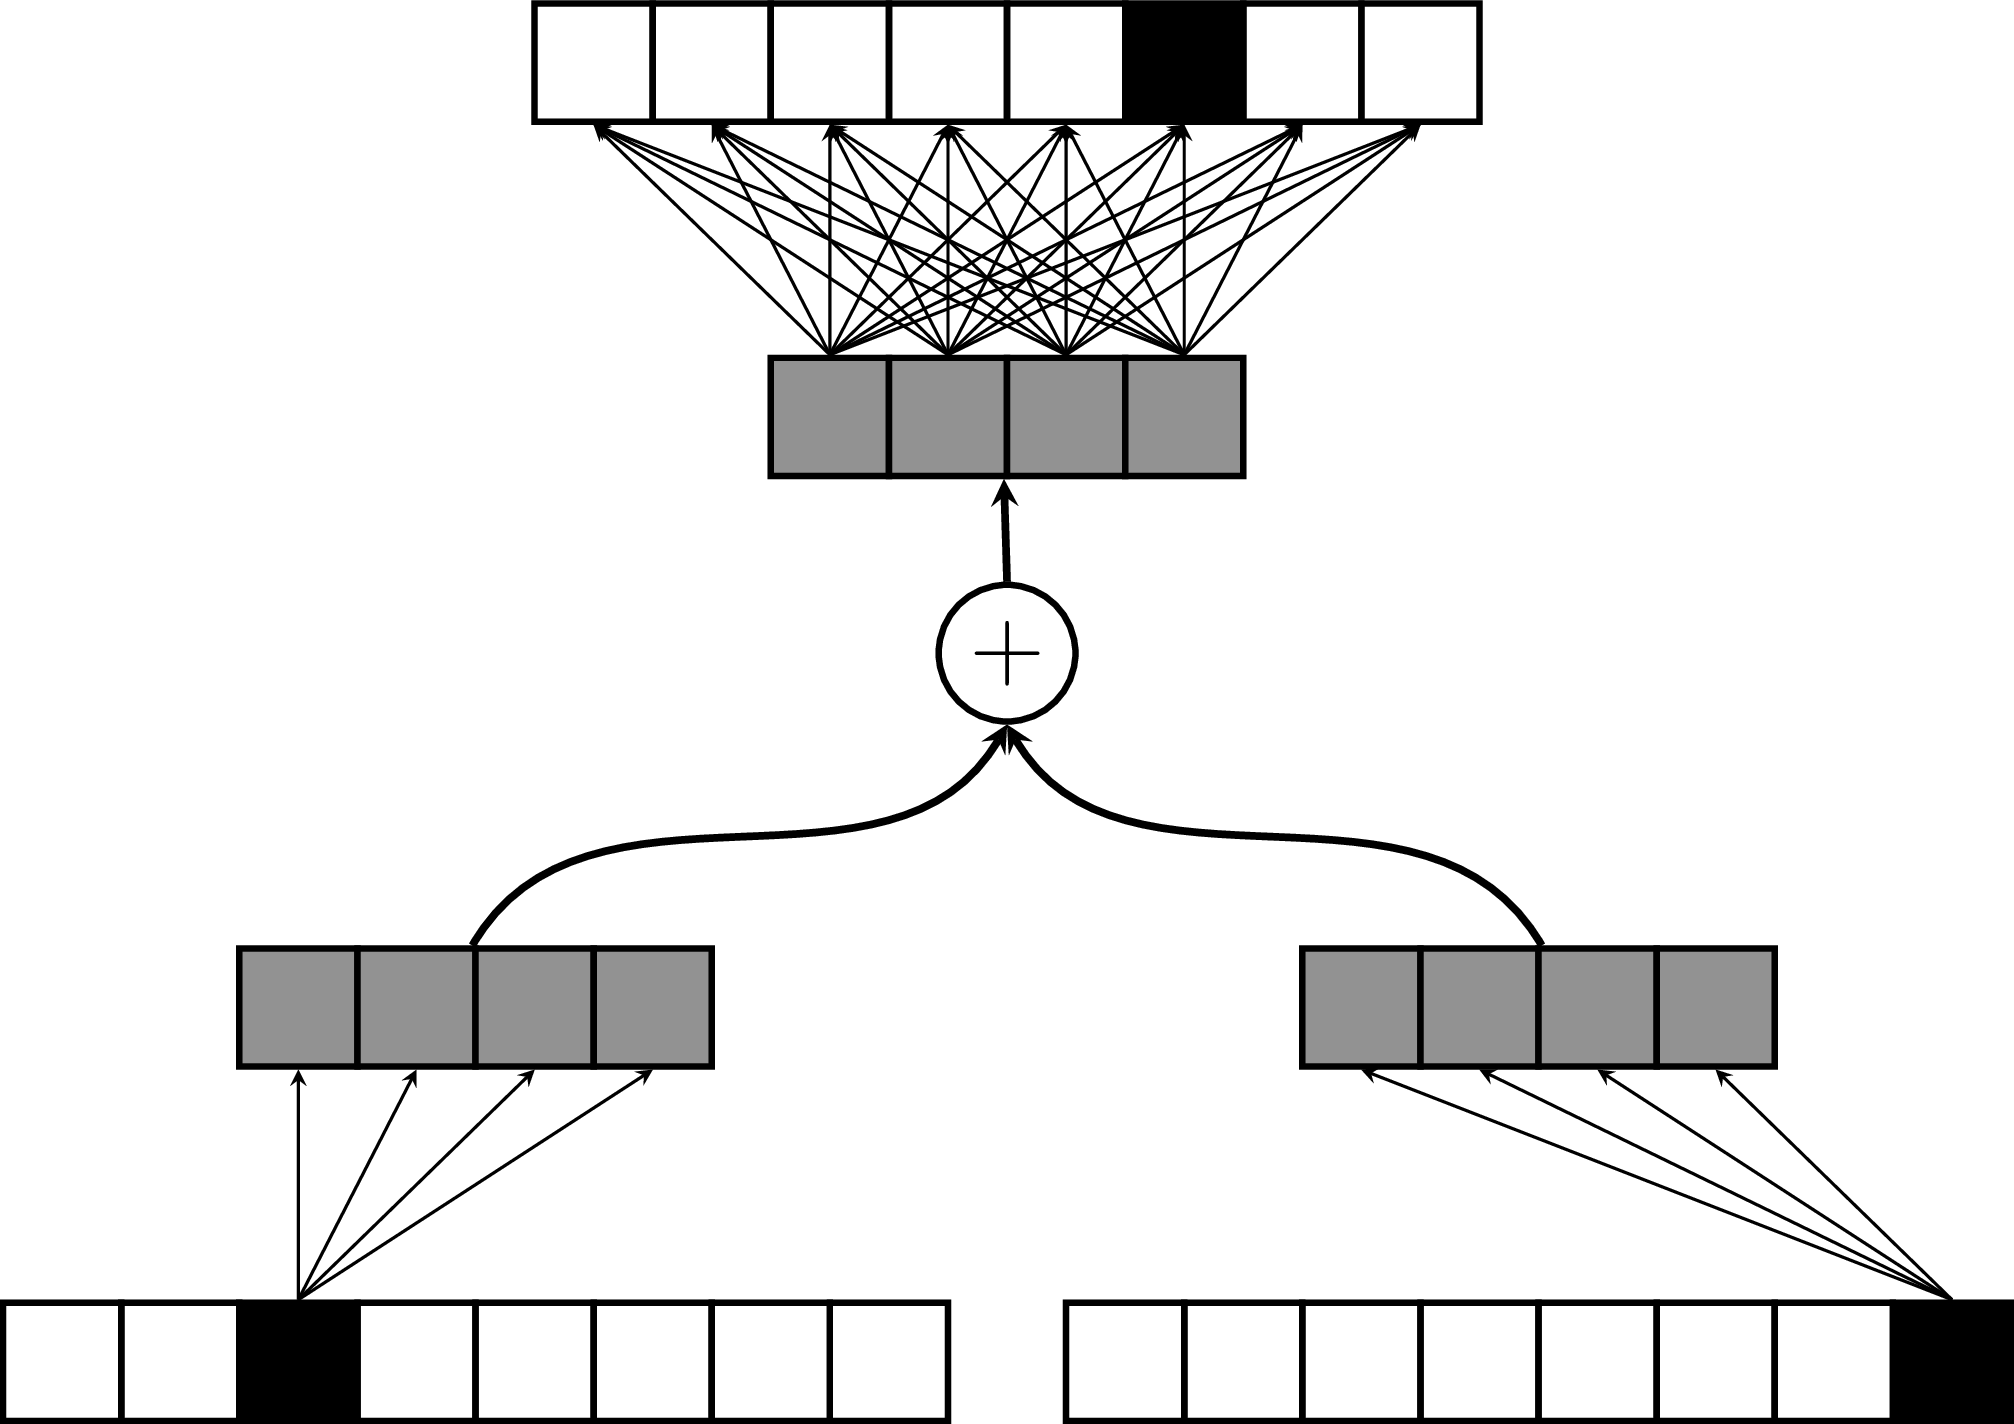
\includegraphics[width=5cm]{cbow_fig.png}
    \caption{}
    \end{subfigure}%
    \begin{subfigure}[t]{0.45\textwidth}
    \centering
    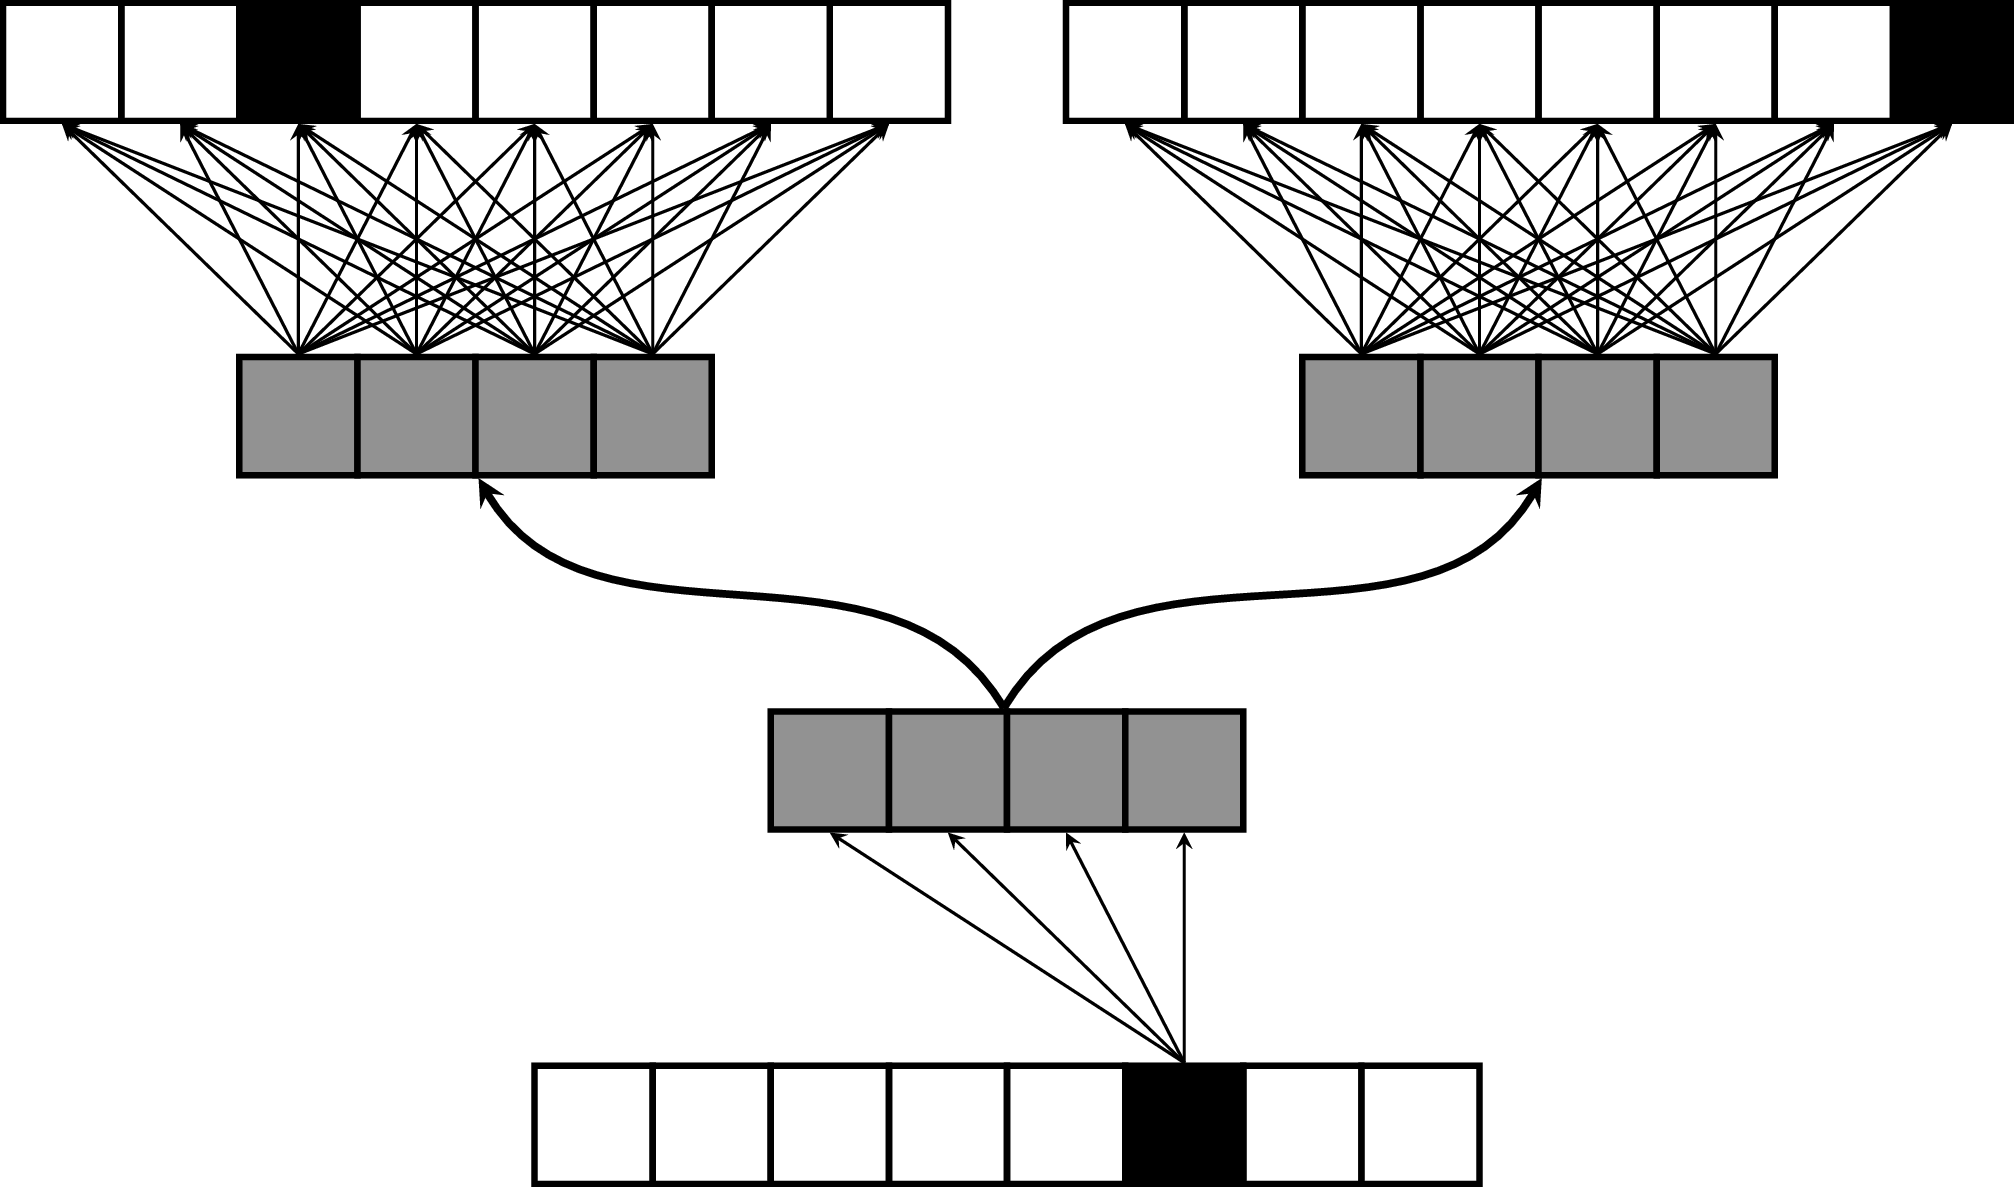
\includegraphics[width=5cm]{skip_gram.png}
    \caption{}
    \end{subfigure}

\caption{The CBOW (left) and skip-gram (right) model architectures for a window of three words. A one-hot vector is depicted as a black square among an array of white squares while an embedding is depicted as an array of gray squares.}
\label{fig:word2vec}
\end{figure}

In this paper, I introduce \texttt{(batter|pitcher)2vec}, an algorithm that adapts representation learning concepts (like those found in \texttt{word2vec}) to a baseball setting. Specifically, the model learns to predict the outcome of an at-bat given a specific batter and pitcher. Unlike many Sabermetrics statistics, \texttt{(batter|pitcher)2vec} learns from "raw" baseball events as opposed to aggregate statistics, which allows it to incorporate additional contextual information when modeling player talent.

\section{Data}
\label{data}

\begin{table}[h]
\caption{The possible at-bat outcomes.}
\centering
\begin{adjustbox}{max width=\textwidth}
    \begin{tabular}{ | l | l | l | l | }
    \hline
    Symbol & Description & Symbol & Description \\ 
    \hline\hline
    1-9 & Out first handled by fielder \# & E1-E9 & Error first handled by fielder \# \\
    \hline
    S1-S9 & Single first handled by fielder \# & K & Strike out \\
    \hline
    D1-D9 & Double first handled by fielder \# & W & Walk \\
    \hline
    DG & Ground rule double & IW & Intentional walk \\
    \hline
    T1-T9 & Triple first handled by fielder \# & BK & Balk \\
    \hline
    HR & Home run & HP & Hit by a pitch \\
    \hline
    \end{tabular}
\end{adjustbox}
\label{table:at_bats}
\end{table}

Play-by-play data for each game from the 2013, 2014, 2015, and 2016 seasons were obtained from the Retrosheet website \parencite{Retro}. Each play description was converted into a tuple consisting of the batter, pitcher, and at-bat outcome; for example, (Mike Trout, Anthony Bass, HR), where HR is the symbol denoting a home run. There are 52 potential play outcomes (see Table~\ref{table:at_bats}), but the model only considers 49 different outcomes because there were no observed instances of doubles first fielded by the catcher, triples first fielded by the catcher, or triples first fielded by the third baseman. The raw training data set consisted of 557,436 at-bats from the 2013, 2014, and 2015 seasons representing 1,634 different batters and 1,226 different pitchers. To ensure an adequate amount of data was available for learning player representations, only the most frequent batters and pitchers involved in 90\% of at-bats were included in the analysis. The final data set consisted of 461,231 at-bats with 524 batters and 565 pitchers.

\section{Model}
\label{model}

\begin{figure}[h]
\centering
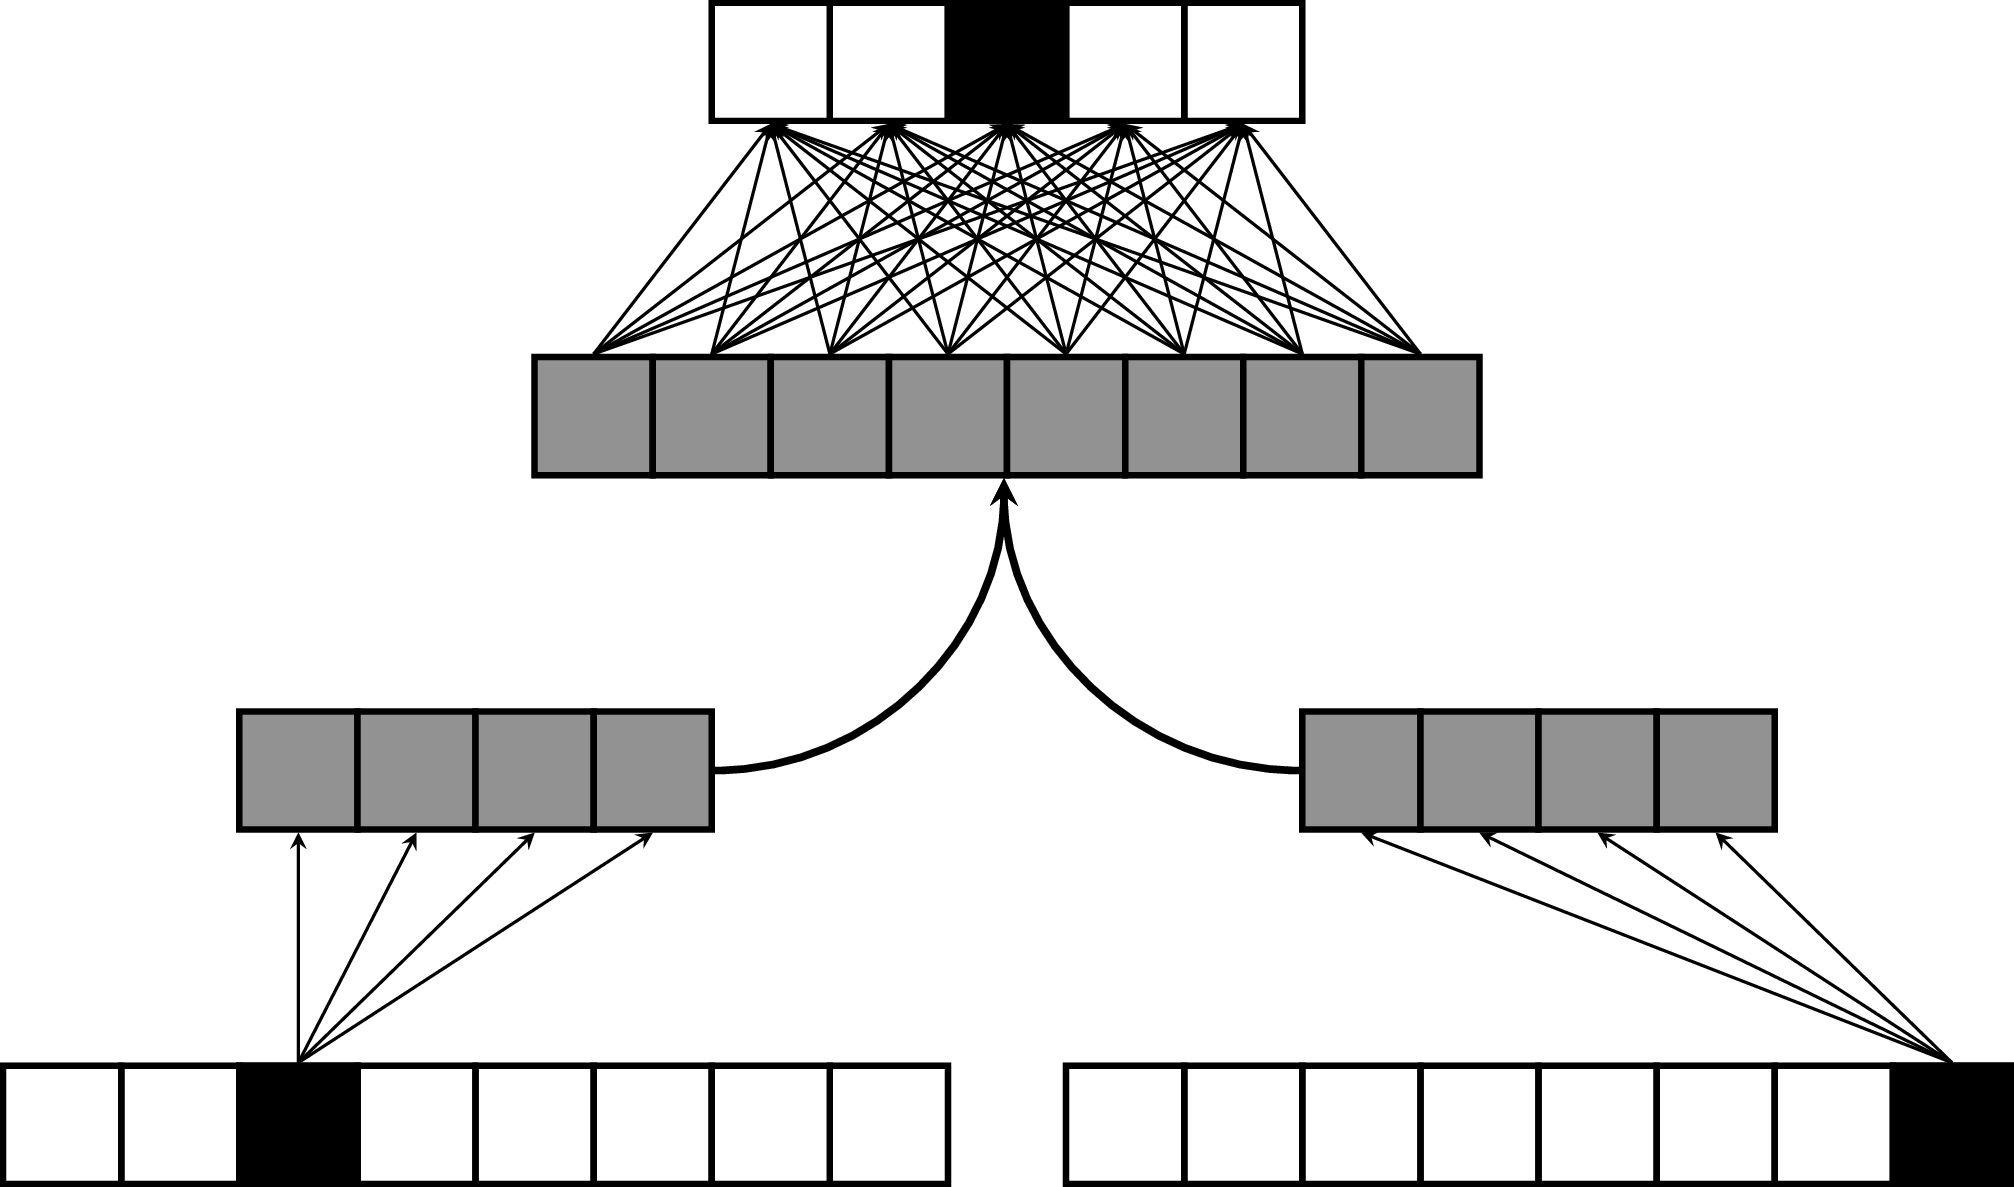
\includegraphics[width=0.75\textwidth,height=\textheight,keepaspectratio]{batter_pitcher_model.png}
\caption{The \texttt{(batter|pitcher)2vec} model architecture.}
\label{fig:batter_pitcher}
\end{figure}

The \texttt{(batter|pitcher)2vec} model architecture can be seen in Figure~\ref{fig:batter_pitcher}, and the similarities between \texttt{(batter|pitcher)2vec} and \texttt{word2vec} should be readily apparent. The model takes one-hot encodings of a batter and pitcher as input and then selects the corresponding player weights from the the batter (\ref{eqn:batter_embedding}) and pitcher (\ref{eqn:pitcher_embedding}) weight matrices, respectively. The player weight vectors are then passed through a "sigmoid"/logistic activation function.

\begin{equation}
\label{eqn:batter_embedding}
w_b = \sigma(W_B \cdot h_b)
\end{equation}

\begin{equation}
\label{eqn:pitcher_embedding}
w_p = \sigma(W_P \cdot h_p)
\end{equation}

Here, $h_b$ is the $N_B$-dimensional one-hot vector (where $N_B$ is the number of batters) for the batter indexed by $b$, $W_B$ is the batter embedding matrix, $\sigma$ is the logistic activation function (i.e., $\frac{1}{1 + e^{-x}}$) and $w_b$ is the batter's embedding. Likewise, $h_p$ is the $N_P$-dimensional one-hot vector for the pitcher indexed by $p$, $W_P$ is the pitcher embedding matrix, and $w_p$ is the pitcher's embedding.

The batter and pitcher embeddings are then concatenated together (\ref{eqn:concat}) and fed into a standard softmax layer (\ref{eqn:output} and \ref{eqn:prob}), which outputs a probability distribution over at-bat outcomes.

\begin{equation}
\label{eqn:concat}
w_{b \oplus p} = w_b \oplus w_p
\end{equation}

\begin{equation}
\label{eqn:output}
z = W_o \cdot w_{b \oplus p} + b_o
\end{equation}

\begin{equation}
\label{eqn:prob}
p(o_i | h_b, h_p) = \frac{e^{z_i}}{\sum_{j=1}^{K} e^{z_j}}
\end{equation}

Here, $o_i$ is the at-bat outcome indexed by $i$ and $K$ is the number of possible at-bat outcomes.

Maximizing the likelihood of this model is equivalent to minimizing the model's average cross entropy (\ref{eqn:entropy}), which is the standard loss function used in machine learning classification tasks and is defined as:

\begin{equation}
\label{eqn:entropy}
\mathcal{L}(D) = \frac{1}{N}\sum_{i=1}^{N}H(p_i,q_i) = -\frac{1}{N}\sum_{i=1}^{N}\sum_{j=1}^{K} p_i(o_j)log(q_i(o_j))
\end{equation}

where $D$ is the training data, $N$ is the number of training samples, $H(p_i,q_i)$ is the cross entropy between the probability distributions $p_i$ and $q_i$, $p_i$ is the true at-bat outcome distribution for training sample $i$, and $q_i$ is the predicted outcome distribution for training sample $i$.

The model was implemented in Keras 2.0 \parencite{Keras2015} and trained on a laptop with 16 gigabytes of RAM and an Intel i7 CPU. The model was optimized using Nesterov accelerated mini-batch gradient descent with the learning rate, momentum, and decay hyperparameters set at $0.01$, $0.9$, and $10^{-6}$, respectively. The model was trained for $100$ epochs and with mini-batches of $100$ samples. The embeddings for both batters and pitchers were nine-dimensional. The code to generate the results described in this paper can be found at \url{https://github.com/airalcorn2/batter-pitcher-2vec}.

\section{Results}
\label{results}

\subsection{Visual inspection of the player embeddings}

Visually inspecting low-dimensional approximations of model embeddings can often provide some intuition for what the model learned. Several plots of the first two principal components of the batter embeddings can be seen in Figure~\ref{fig:batter_traits}. A number of trends are readily apparent; for example, left-handed hitters are clearly distinguishable from right-handed hitters, and batters with high single rates are antipodal to batters with low single rates (a similar pattern is visible for home run rates). At the least, \texttt{(batter|pitcher)2vec} appears to be capable of capturing the information contained in standard baseball statistics.

\begin{figure}[h]
\captionsetup[subfigure]{labelformat=empty}
\centering
    \begin{subfigure}{0.5\linewidth}
    \centering
    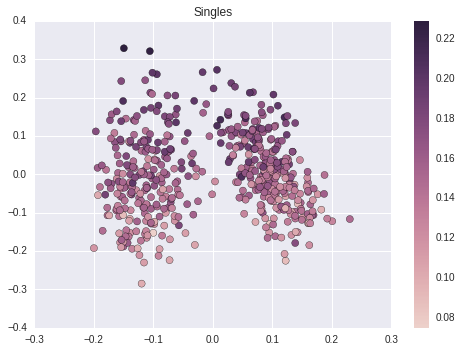
\includegraphics[width=1\linewidth]{batter_single.png}
    \caption{}
    \end{subfigure}%
    \begin{subfigure}{0.5\linewidth}
    \centering
    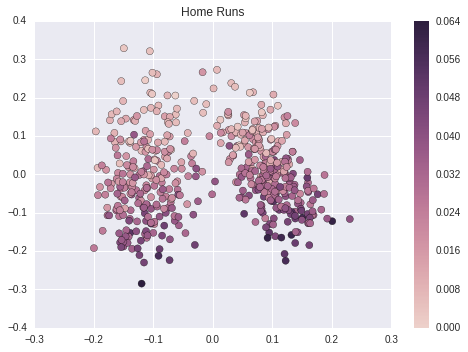
\includegraphics[width=1\linewidth]{batter_hr.png}
    \caption{}
    \end{subfigure}\\[1ex]

    \begin{subfigure}{0.5\linewidth}
    \centering
    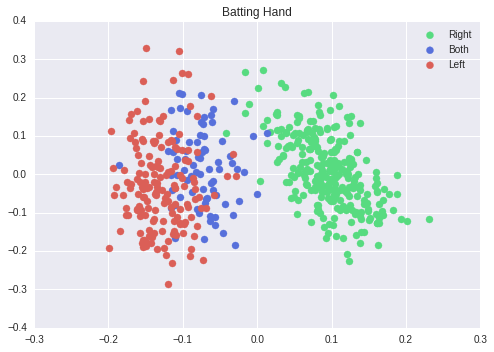
\includegraphics[width=1\linewidth]{batter_hand.png}
    \caption{}
    \end{subfigure}
\caption{Plots of the first two principal components of the batter embeddings colored by various batter qualities.}
\label{fig:batter_traits}
\end{figure}

\subsection{Nearest neighbors}

Inspecting the neighborhoods of individual embeddings can also yield a deeper understanding of the model. Two-dimensional embeddings of the batter and pitcher embeddings were obtained using the t-SNE algorithm \parencite{VanderMaaten2008} and can be seen in Figure~\ref{fig:tsne}. Intriguing player clusterings are readily apparent, with close pairs including: Mike Trout/Paul Goldschmidt, Dee Gordon/Ichiro Suzuki, and Aroldis Chapman/Dellin Betances.

\begin{figure}[h]
\captionsetup[subfigure]{labelformat=empty}
\centering

    \begin{subfigure}[b]{0.75\textwidth}
    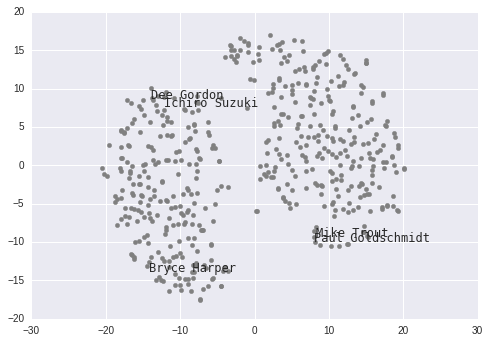
\includegraphics[width=1\linewidth]{batter_tsne.png}
    \caption{}
    \end{subfigure}

    \begin{subfigure}[b]{0.75\textwidth}
    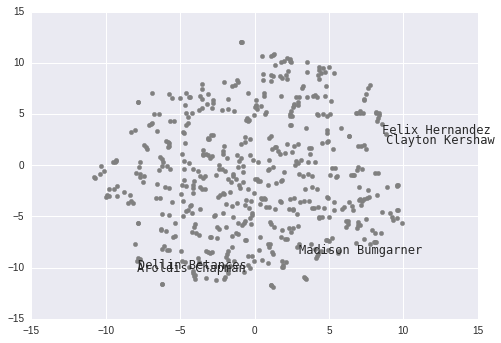
\includegraphics[width=1\linewidth]{pitcher_tsne.png}
    \caption{}
    \end{subfigure}

\caption{Two-dimensional t-SNE embeddings of the learned batter (top) and pitcher (bottom) representations.}
\label{fig:tsne}
\end{figure}

When calculating nearest neighbors in the raw embedding space, Paul Goldschmidt is indeed Mike Trout's nearest neighbor; an unsurprising result considering how each athlete is known for his rare blend of speed and power \parencite{Kory2015}. Similarly, Ichiro Suzuki is Dee Gordon's nearest neighbor, which is to be expected as both have a reputation for being able to get on base \parencite{Sullivan2015}. Notably, when clustering players using common MLB stats (e.g., HRs, RBIs), Paul Goldschmidt is not among Mike Trout's ten nearest neighbors, nor is Ichiro Suzuki among Dee Gordon's ten nearest neighbors.

For pitchers, Craig Kimbrel is Aroldis Chapman's nearest neighbor, which is unsurprising considering both are known as elite closers with overpowering fastballs \parencite{Mirsky2016}. Similarly, Félix Hernández, much like his two nearest neighbors, Jean Machi and Carlos Carrasco, is known for having a pitch with incredible movement in his repertoire \parencite{Buchanan2015, Romano2015, Berg2016}. Other nearest neighbors are not as immediately obvious, for example, Clayton Kershaw and Craig Stammen (although, Zack Greinke is Kershaw's second nearest neighbor), but a method like \texttt{(batter|pitcher)2vec} could potentially reveal surprising similarities between players who are not considered similar by human standards.

\subsection{Opposite-handed dopplegängers}

One of the most fascinating properties of effective word embeddings is their analogy capabilities \parencite{Mikolov2013a}. For example, when using \texttt{word2vec} word embeddings, subtracting the vector for "France" from the vector for "Paris" and then adding the vector for "Rome" produces a vector that is very close to the vector for Rome, which corresponds to the analogy Paris : France :: Rome : Italy \parencite{Mikolov2013a}.

To investiage the algebraic properties of the \texttt{(batter|pitcher)2vec} embeddings, the average embeddings were calculated for all left-handed and right-handeded batters, respectively, and then subtracted from select players to generate opposite-handed dopplegängers. For example, subtracting the average left-handed batter embedding from the embedding for Mike Trout (a right-handed batter) embedding produces a vector with Chris Davis, David Ortiz, and Bryce Harper (all powerful left-handed batters) as the three nearest neighbors, suggesting the algebra hypothesis holds (see \parencite{Spector2016} for a discussion of the similarities between Mike Trout and Bryce Harper). Similarly, Tyler Saladino appears to be an appropriate candidate for Dee Gordon's right-handed dopplegänger \parencite{Chamberlain2017}.

\subsection{Modeling previously unseen at-bat matchups}

Neural network representations are theoretically interesting because they suggest the models are learning "causal" factors from inputs when they are able to generalize (or transfer) well \parencite{RepresentationLearning}. In the case of \texttt{(batter|pitcher)2vec}, accurately modeling at-bat outcome distributions for unseen batter and pitcher pairs would indicate the model is extracting truly meaningful baseball qualities during learning. To test the model, at-bat outcomes were collected from the 2016 season for previously unseen matchups that included batters and pitchers from the training set. In all, there were 21,479 previously unseen matchups corresponding to 51,580 at-bats.

A naïve prediction strategy was used as a baseline for comparison to \texttt{(batter|pitcher)2vec}. For any given batter, the expected outcome distribution was defined as:

\begin{equation}
\label{eqn:batter_naïve}
p(o_i|b_j)=\frac{c_{i,j} + r_i}{\sum_{k=1}^{K} c_{j,k} + 1}
\end{equation}

where $o_i$ denotes the outcome indexed by $i$, $b_j$ represents the batter indexed by $j$, $c_{i,j}$ is the number of times the batter indexed by $j$ had an at-bat resulting in the outcome indexed by $i$ in the training data, $r_i$ is the proportion of all at-bats that resulted in the outcome indexed by $i$ in the training data, and $K$ is the number of outcomes. Essentially, the procedure adds one at-bat to each batter's data, but distributes the probability mass of that single at-bat across all possible outcomes based on data from all batters. $r_i$ can thus be considered a type of "prior" or smoothing factor. $p(o_i|t_j)$ will be similarly defined for pitchers. The naïve expected outcome distribution for a given batter ($b_j$) and pitcher ($t_k$) matchup is thus defined as:

\begin{equation}
\label{eqn:naïve}
p(o_i|b_j,t_k) = \frac{p(o_i|b_j) + p(o_i|t_k)}{2}
\end{equation}

The cross entropy was calculated for each at-bat in the test set using both the naïve approach and \texttt{(batter|pitcher)2vec}. The naïve approach produced an average cross entropy of $2.8113$ on the test set while \texttt{(batter|pitcher)2vec} produced a significantly ($p < 0.001$) lower average cross entropy of $2.7848$, a $0.94\%$ improvement. But is an improvement of only $0.94\%$ over the baseline particularly impressive? In comparison, a multinomial logistic regression model (Figure~\ref{fig:log_reg}) trained and tested on identical data sets produced an average cross entropy of $2.8118$, which is slightly worse than the naïve approach. \texttt{(batter|pitcher)2vec} thus appears to be exceptional in its ability to model at-bat outcome distributions for previously unseen matchups.

\begin{figure}[h]
\centering
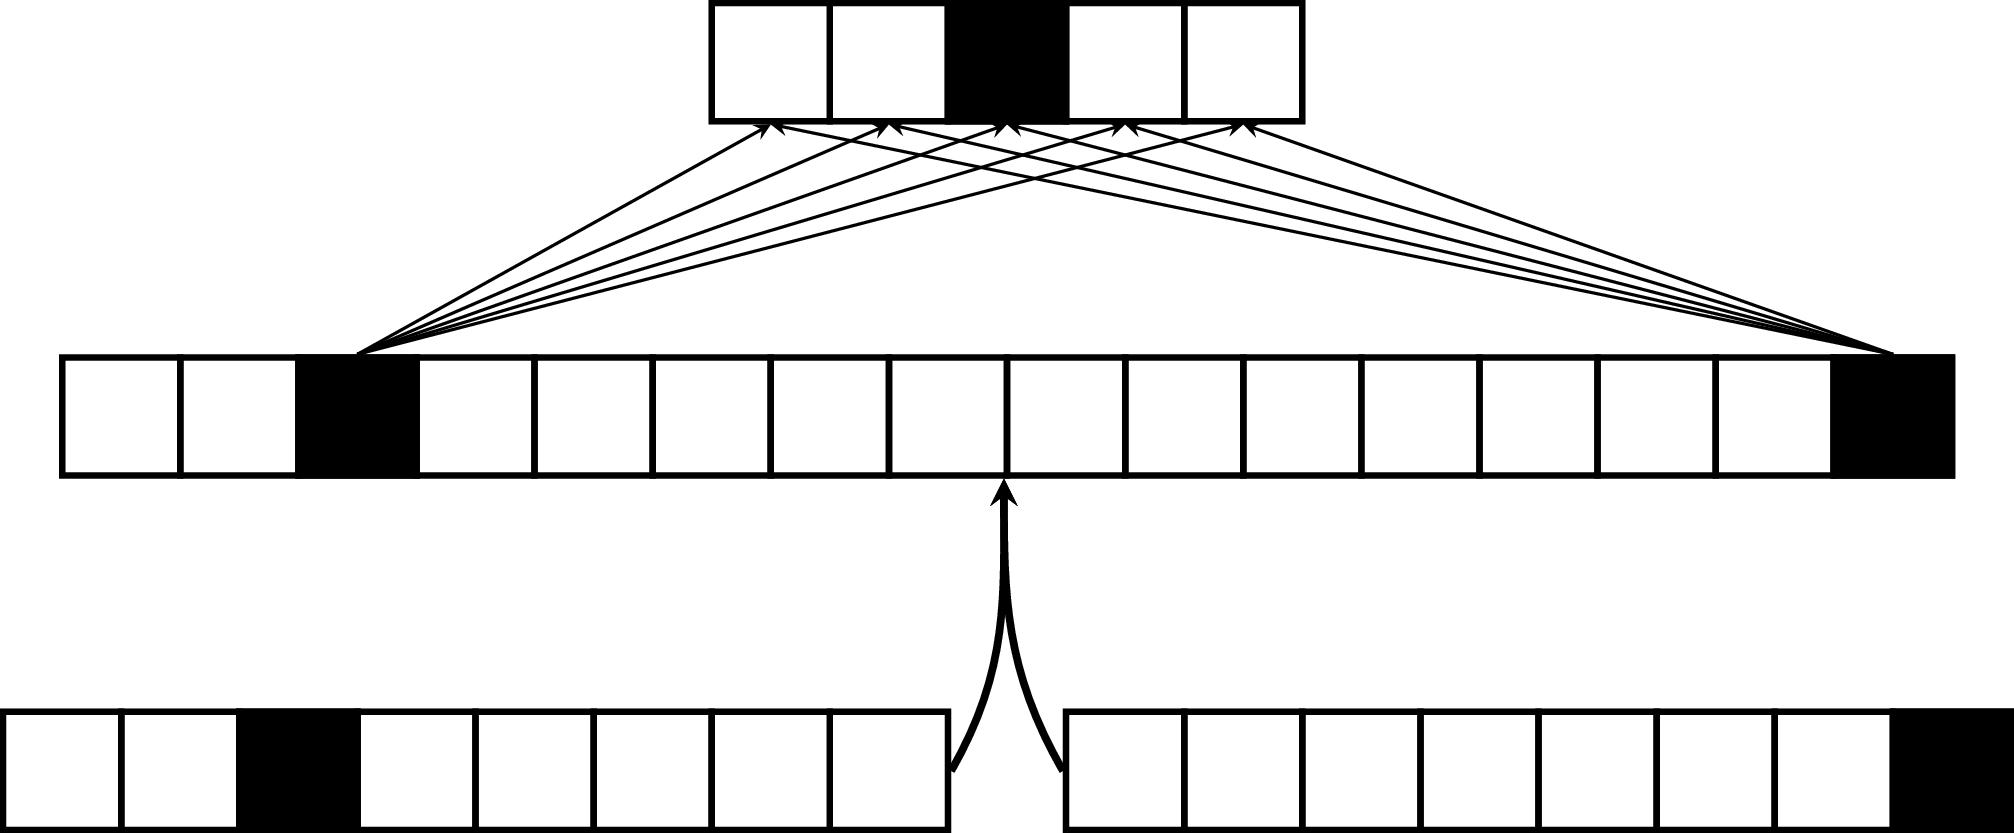
\includegraphics[width=0.75\textwidth,height=\textheight,keepaspectratio]{logistic_regression.png}
\caption{A graphical model depiction of multinomial logistic regression.}
\label{fig:log_reg}
\end{figure}

\section{Future directions}
\label{future}

These results suggest neural embedding architectures offer a principled means of modeling talent from "raw data", i.e., without resorting to ad hoc statistics. Further, neural architectures are extremely flexible, which makes them excellent candidates for modeling discrete elements in a variety of sports settings. Modifying \texttt{(batter|pitcher)2vec} to predict PITCHf/x measurements as opposed to discrete outcomes could be fruitful as PITCHf/x data would likely convey more information about a player's physical characteristics. Another potentially interesting adaptation of \texttt{(batter|pitcher)2vec} would be modeling the pitcher's supporting defense by including the pitcher's team as one of the model inputs (mirroring the approach taken with \texttt{doc2vec} in \parencite{Le2014}).

Applying \texttt{(batter|pitcher)2vec} to minor league baseball players would present the opportunity to then train a second model that learns a mapping from a player's minor league representation to his MLB representation, which conceptually resembles the cross-modal model developed by \parencite{}. Such a model could be used for scouting purposes to identify neighboring MLB players of the prospect's mapped embedding.

The player embeddings may also allow for better trade evaluations. For example, swapping the players in a proposed trade and "back simulating" games from earlier in the season could allow a team to assess how many more wins (or losses) they would have obtained with the candidate player on the roster.

Finally, interesting applications of \texttt{(batter|pitcher)2vec}-like architectures are likely possible in sports other than baseball, for example, modeling National Football League offenses and defenses as proposed by \parencite{Alcorn2016}.

\subsubsection*{Acknowledgments}

I would like to thank my colleague Erik Erlandson for his suggestion to investigate opposite-handed dopplegängers.

\printbibliography

\end{document}